\documentclass[
 aip,
 jcp,
 numerical ,
 reprint, %onecolumn
]{revtex4-1}

\usepackage{braket}
\usepackage{graphicx}
\usepackage{dcolumn}
\usepackage{bm}
\usepackage{array}
\usepackage{booktabs}
\usepackage{multirow}
\usepackage{rotating}
\usepackage{amsmath}
\usepackage{epsfig}
\usepackage{appendix}
\usepackage{color}
\usepackage{natbib}
\usepackage{makeidx}
%\bibliographystyle{abbrv}
%\def\etal{\mbox{et al.}}

\begin{document}

\title{N-electron valence state perturbation theory based on density matrix renormalization group reference functions, with applications to chromium dimer and photovoltaic polymers}
\author{Sheng Guo, Mark A. Watson, Weifeng Hu, Qiming Sun, Garnet Kin-Lic Chan}
\affiliation{Department of Chemistry, Princeton University, Princeton, New Jersey 08544, USA}

\begin{abstract}

The second order n-electron valence state perturbation theory (NEVPT2) is a relatively cheap way to deal dynamic correlation without intruder state problem or level shift, while density matrix renormalization group (DMRG) is able to deal static correlation with a large active space and to provide reference wave functions needed in multireference perturbation theories.
We present a method to combine DMRG and NEVPT2 (DMRG-NEVPT2) through the a general algorithm to compute high order reduced density matrices for DMRG wave function. The capacity of DMRG-NEVPT is demonstrated for calcualtions of chromium dimer potential energy curve and excited states energy of poly(p-phenylene vinylene).

%\begin{keywords}
%DMRG; dynamic correlation; chromium dimer, PPV
%\end{keywords}\bigskip
\end{abstract}

\date{\today}

\maketitle


\section{introduction}

The density matrix renormalization group \cite{white_density_1992,white_density-matrix_1993} has made it accessible to employ large active spaces 
for electronic structure problems in quantum chemistry. Nowadays, it has become quite straightforward to use DMRG as a robust numerical solver for 
static electron correlation problems. Examples are benchmark solutions of small molecules\cite{chan_highly_2002}, transition metal 
clusters\cite{sharma_low-energy_2014, olivares-amaya_ab-initio_2015}, also molecular crystals\cite{yang_ab_2014}. 

In chemical systems, electron interaction across large energy scales brings many other important chemistry, such as low-lying excited states in 
conjugated polymers, high-spin ground state in transition metals complexes. Qualitative and quantitative characterizations of 
these systems generally require correlating many electrons within a large number of orbitals. Direct treatment of such problem is generally 
impossible, but indirect methodology can apply, for example, by expanding the electron correlation outside active spaces. So far, there are 
methods which follow with this strategy with using large active spaces, for example, to apply perturbation theory to a large active space, or 
perform canonical transformation to get an effective Hamil
%On the other hand, dynamic electron correlation is crucial in chemical dynamic processes, which in general involves electron correlation dynamics within a large range of orbitals. 
The DMRG method has been embedded with the second-order perturbation theory\cite{kurashige_second-order_2011, sharma_communication:_2014}, 
complete active space perturbation theory (CASPT), and canonical transformation(CT)\cite{neuscamman_review_2010}, etc., to be extended for dynamic correlation. In these methods, high order particle density matrices are generally needed, which are theoretically straightforward yet computationally non-trivial to compute.

In this work, we implemented second order $n$-electron valence state perturbation theory based of DMRG wavefunction (DMRG-NEVPT2) and 
apply it to the quasi-one dimensional  photovoltaic molecule poly(p-phenylene vinylene) (PPV) and chromium dimer. PPV has always been 
of great interest by photophysists and photochemists, as it is well known for its charge-transfer properties upon photoexcitations. Due 
to the highly conjugated structure in PPV, the first optically bright state $1^{1}B_{u}$ whose polaronic feature is suggested to be 
responsible for the charge-transfer behavior, is estimated to lie below the $2^{1}A_{g}$ with a small gap of 0.7eV. For a more accurate 
estimate of the energy order and energy gaps, including the dynamic correlation can be considered as an effective way. %need to say something more...

%In this work, we introduce an algorithm which generally applies to any order of (transition) particle density matrices for DMRG wave functions. We first give a brief review on the DMRG method in Sec. Further we present a general algorithm to evaluate any order particle density matrices in Sec.. We show the application of this algorithm in the DMRG-NEVPT2 method, to study the static and dynamic correlation effects of photovoltaic polymer PPV in Sec.

\section{Theories}


\subsection{DMRG wavefunction and optimization algorithm}

As with other approximate wavefunction methods in quantum chemistry, DMRG is based on an approximate wvefunction ansatz. It is the matrix product state (MPS).
A MPS is a non-linear wavefunction, built from contraction of tensors for each orbital in the basis. Limited by the dimension of tensors, called bond dimension, $M$, MPS could only explore a small subspace of Hilbert space. By increasing $M$, the MPS ansatz will give full configuration interaction (FCI) results. DMRG is a combination of renormalization and truncation algorithms to find a variational and optimal MPS. 
In practice, two types of MPS are often used in DMRG calculations: one-site and two-site MPS. 

The one-site MPS is defined as

\begin{equation}
  \ket{\Psi}= \sum_{\substack{n_1, n_2\cdot\cdot\cdot n_p\cdot\cdot\cdot n_k}} {\bf A}^{n_1}{\bf A}^{n_2}\cdot\cdot\cdot {\bf A}^{n_{p}} \cdot\cdot\cdot{\bf A}^{n_k}
\end{equation}

Here, $n_i$ is the occupacy of orbital $i$, one of $ \{\ket{}, \ket{\uparrow}, \ket{\downarrow}, \ket{\uparrow\downarrow}\}$ and $k$ is the number of orbitals. 
For a given $n_i$, ${\bf A}^{n_i}$ is $M\times M$ matrix, except that the first and last ones. For ${\bf A}^{n_1}$ and ${\bf A}^{n_k}$, their dimensions are $1\times M$ and $M\times 1$ respectively. 
This ensures that for a given string $n_1n_2\cdots n_k$, a slater determinant, the ${\bf A}^{n_1}{\bf A}^{n_2}\cdots{\bf A}^{n_k}$ yields a scalar, the coefficient of the determinant $\ket{n_1n_2\cdots n_k}$

Similarly, the two-site MPS is defined as

\begin{equation}
  \ket{\Psi}= \sum_{\substack{n_1, n_2\cdot\cdot\cdot n_p\cdot\cdot\cdot n_k}} {\bf A}^{n_1}{\bf A}^{n_2}\cdot\cdot\cdot {\bf A}^{n_{p},n_{p+1}} \cdot\cdot\cdot{\bf A}^{n_k}
\end{equation}

In DMRG sweep algorithm, $\bra{\Psi}\hat{H}\ket{\Psi}$ is variational optimized. And only a single tensor ($A^{n_i}$ for an one-site MPS or $A^{n_i, n_{i+1}}$ for a two-site MPS) in the MPS is updated during the sweep at site $i$. It can be considered as solving eigenvalue problem of an effective Hamiltonian, which is a $4M^2\times 4M^2$ matrix. 
The multiplication between this effective Hamiltonian and a MPS is usually computed from $O(k^2)$ operators built on different subspaces of active orbitals spaces. The cost scaling is $O(k^2M^3)$ for this eighenvalue problem for one tensor and is $O(k^3M^3)$ for a whole sweep optimization. 

Compared to an one-site MPS, a two-site MPS has more variational freedom and is able to change quantum numbers during the sweep. It helps avoid local minimums. However, the two-site MPS has N-representation problem: the converged two-site MPS is still different at different position of the sweep.\cite{zgid_obtaining_2008} Based on a two-site MPS, expectation values, for example reduced density matrix, which often used to characterize a state and is essential for dynamic correlation calculations, have no unique results. 
Therefore, the strategy, ``two-site to one-site'' (a two-site MPS optimization followed by an one-site one), is widely used\cite{olivares-amaya_ab-initio_2015}. 
















%A mixed canonical form of MPS at site $p$ is 
%
%\begin{eqnarray}
%    \ket{\Psi_{MPS}}=&& \sum_{\substack{n_1\cdot\cdot\cdot n_p\cdot\cdot\cdot n_k\\l_1\cdot\cdot\cdot l_{p-1},r_p\cdot\cdot\cdot r_{k-1} }} L^{n_1}_{l_1}\cdot\cdot\cdot L^{n_{p-1}}_{l_{p-2},l_{p-1}} C^{n_p}_{l_{p-1},r_p}\nonumber\\
%&&  R^{n_{p+1}}_{r_p,r_{p+1}}\cdot\cdot\cdot R^{n_k}_{r_{k-1}}
%\times\ket{n_1\cdot\cdot\cdot n_p \cdot\cdot\cdot n_k}
%\end{eqnarray}
%
%$L^{n_i}_{l_{i-1},l_i}$ is for the sites on the left of p and $R^{n_i}_{r_{i-1},r_i}$ is for the sites on the right of $p$. $n_i$ is one of four single site states \{$\ket{0},\ket{\uparrow},\ket{\downarrow},\ket{\uparrow\downarrow}$\}. (In spin-adapted dmrg code, block, (citation here) only three states are necessary.). The dimension of bond index $l_i$ or $r_i$ (M) is the number of kept renormalized states. MPS is more accurate with a higher M. L and R site functions are canonical by following definition,
%
%\begin{equation}
%\sum_{n_q,l_{q-1}} L^{n_q}_{l_{q-1},l_q} L^{n_q}_{l_{q-1},l'_q} = \delta_{l_q,l'_q}
%\end{equation}
%
%\begin{equation}
%\sum_{n_q,l_q} R^{n_q}_{r_{q-1},r_q} R^{n_q}_{r'_{q-1},l_q} = \delta_{r_{q-1},r'_{q-1}}
%\end{equation}
%
%Combine L site functions and occupation number basis for the left block, which is formed by the sites on the left of p, we get
%
%\begin{eqnarray}
%\ket{l_{p-1}} = &&\sum_{\substack{n_1,n_2,..n_{p-1}\\l_1,l2,...,l_{p-2}}} L^{n_1}_{l_1}L^{n_2}_{l_1,l_2}\cdot\cdot\cdot L^{n_{p-1}}_{l_{p-2},l_{p-1}}\nonumber\\
%&&\times \ket{n_1,n_2,..,n_{p-1}}
%\end{eqnarray}
%\begin{eqnarray}
%\ket{r_{p}} = &&\sum_{\substack{n_{p+1},..n_{k-1},n_k\\r_{p+1},...,r_{k-2},r_{k-1}}} R^{n_{p}}_{r_{p},r_{p+1}}\cdot\cdot\cdot R^{n_{k-1}}_{r_{k-2},r_{k-1}}R^{n_k}_{r_k} \nonumber\\
%&&\times \ket{n_{p+1},...,n_{k-1},n_k}
%\end{eqnarray}
%
%With the renormalized basis definied above, wavefunction at site $p$ is
%
%\begin{equation}
%\ket{\Psi} = \sum_{n_p,l_{p-1},r_p} C^{n_p}_{l_{p-1},r_p} \ket{l_{p-1},n_p,r_p}
%\end{equation}


\subsection{Reduced density matrix (RDM)}


From now on, when we refer MPS, it means an one-site MPS, because it is needed in reduced density matrix and dynamic correlation calculations.
%Our focus is how to calculate dynamic correlations based on a DMRG wavefunction ( an one-site MPS), rather than how to get this wavefunction. 

The 2-RDM is defined in this way

\begin{equation}
\gamma_{i,j,k,l}=\sum_{\sigma,\tau} \bra{\Psi}a^\dagger_{i,\sigma}a^\dagger_{j,\tau}a_{k,\tau}a_{l,\sigma}\ket{\Psi}
\end{equation}

It is similar for the higher order reduced density matrix.

%An efficient way to compute RDM elements is to partition operators into left and right block operators as 
%
%\begin{equation}
%  \bra{\Psi} \hat{O}_{LR} \ket{\Psi} = (-1)^P \sum_{l',r',l,r} c^*_{l',r'} \bra{l'}\hat{O}_{L}\ket{l} \bra{r'}\hat{O}_{R}\ket{r} c_{l,r} = Tr(X^TY)
%\end{equation}
%where 
%  $X_{l,r'} =  \sum_{l'} c^*_{l',r'} \bra{l'}\hat{O}_{L}\ket{l} $ , 
%  $Y_{l,r'} =  \sum_{l'}  \bra{r'}\hat{O}_{R}\ket{r} c_{l,r}$
%  and sign $(-1)^P$ is caused by the permutation among the elementary operators and renormalized basis. Computational scaling for $Tr(X^TY)$ operators of $k^{2N}$ RDM elements( k is the number of active orbital and N is the order of the RDM) is $O(k^{2N}M^2)$. The cost for compuation of $X$ and $Y$ depends on how to partition $O_{LR}$ into $O_L$ and $O_R$. In our implementation, we developed a scheme to automatically generate different types of $O_L$ and $O_R$ and the loop to compute RDM elements.
%
%The left block is usually divided into a system block ($\mathcal{S}$), which is expanded during the sweep and the operators on it can be easy build on the flying and a dot block  ($ \mathcal{D}$), where operators is extremely simple and cheap. The right block is the environment-block ($\mathcal{E}$), where operators needed to be precomputed and stored (usually on disk). 


It is not affordable to build and store $k^{2N}$ operators used in N-RDM.
And for RDM, the expectation value rather than the operators needed. There is no need to build these complicate operators.
One efficient way is to distribute the indices (orbital label) $i,j,k,l$ among different orbital subspace for diferent blocks in DMRG.\cite{ghosh_orbital_2008,zgid_density_2008} 
The complicate operators are the tensor product of small operators on different blocks. If small operators are contracted with the wave function before doing tensor product. The tensor product will become dot product of operators. It is much cheaper. Below are the details.

  Operators like $\hat{a}^\dagger_i\hat{a}^\dagger_j\dots \hat{a}_m\hat{a}_n\dots$ can be permuted into a form like $\hat{o}_{i'}\hat{o}_{j'}\dots \hat{o}_{m'}\hat{o}_{n'}$, with $i'\le j'\le \dots \le m' \le n'$ and $\hat{o}$ is $\hat{a}$ or $\hat{a}^\dagger$. A string with $N$ $\hat{a}$ and $N$ $\hat{a}^\dagger$ determines the type of the operator. 
We call it ``type pattern''. 
Then the string is split into several small pieces according to blocks (orbital subgroups) in DMRG sweep. 

There are three blocks in DMRG sweep algrithom.
The system block ($\mathcal{S}$) is expanded during the sweep and the operators on it can be easy build on the flying. The dot block ($\mathcal{D}$) is composed of a single site and its operators are extremely simple and cheap. The environment block ($\mathcal{E}$) was computed from $\mathcal{S}$ in previous sweep in reverse direction, and its operators needed to be precomputed and stored (usually on disk). 
The $2N$ orbital labels of $\hat{O}$ is needed to be partitioned onto the three blocks. It is computational favorable to put more orbital labels on $\mathcal{D}$ and put few orbital labels on $\mathcal{E}$. And the numbers of orbital labels on $\mathcal{S}$ and $\mathcal{E}$ need to be balanced, otherwise number of operators on one block will be extremely big. For most RDM element (not for element like $\gamma_{0,0,0,0}$), at least one orbital label could be put on $\mathcal{D}$ and at most $N-1$ orbital labels on $\mathcal{E}$ by change the position of the dot site. The set \{$n_\mathcal{S}$,$n_\mathcal{D}$,$n_\mathcal{E}$\} determines the numbers of orbital labels on different blocks. It is called ``number pattern''. In general, every number pattern is valid if the number of orbital labels on $\mathcal{S}$ is no more than $N$, that on $\mathcal{D}$ is no more than 4 and that on $\mathcal{E}$ is no more than $N-1$, except the edge cases for the first step and last step in the sweep (in the appendix).
And nearly every ``type pattern'' could be combined with all ``number patterns'' if with some restrictions (in appendix).   

With above process, the types of operators needed on $\mathcal{S}$, $\mathcal{D}$, and $\mathcal{E}$ are determined for each pattern ( ``type pattern'' and ``number pattern''). Loop the orbital labels of operators, we can build all operators we need. There are about $O(N^k)$ operators, most of which are on $\mathcal{S}$.
  The computation for generate these operators are $O(k^NM^3)$ for one step at the sweep and are $O(k^{N+1}M^3)$ in total.   



  After building operators on each block, $\hat{O}^S$, $\hat{O}^D$, $\hat{O}^E$, combine $\hat{O}^S$ and $\hat{O}^D$ into $O^L$, a big left block $\mathcal{S}\otimes \mathcal{D}$. (Combining $\mathcal{E}$ and $\mathcal{D}$ only for RDM calcualtions is also feasible.) The $\mathcal{E}$ is the right block.
  RDM element $\gamma = \sum_{l,r}\sum_{l',r'} c_{l,r} O^{L}_{l,l'} O^R_{r,r'}c_{l',r'}$ , with $\ket{\Psi} = c_{l,r}\ket{l}\ket{r}$, can be computed in two step. (1) $X_{r,r'} = \sum_{l}\sum_{l'} c_{l,r} O^{l,l'} c_{l',r'}$. (2) $\gamma = \sum_{r,r'} X_{r,r'} O^R_{r,r'}$.
  The reason for contracting wave function with $O^L$ first is that the dimension of $O^L$ is $4M$ while the dimension of $O^R$ is $M$.
  The number of operation required for forming X is $O(k^{N+1}M^3)$ and that for dot product between $X$ and $O^R$ is $O(k^{2N}M^2)$. 
  The computations for N-RDM are $O(k^{N+1}M^3+k^{2N}M^2)$.




  %The types of operators on different blocks are also determined automatically. In N-RDM, $N$ $\hat{a}^\dagger$ and $N$ $\hat{a}$ form strings with different orders. They represent different type of $O_{LR}$.
  %The strings are partitioned into three parts according to number of operators in different blocks. This process forms 'patterns' (combinations of different type operators) for the RDM calculations. For exampke, in 2-RDM, for $\hat{a}^\dagger_i\hat{a}^\dagger_j\hat{a}_k\hat{a}_l (i\le j\le k\le l)$ type operators with number of indices partition 2-1-1, all $\hat{a}^\dagger_i\hat{a}^\dagger_j (i\le j)$ operators on $\mathcal{S}$ should be combined with each of $\hat{a}_l$ operators on $\mathcal{E}$ and the only one of $\hat{a}_k$ operator on $\mathcal{D}$. 
  %In order to build operators and corresponding intermedaite ($X$ or $Y$) and to reuse them, operators on $\mathcal{S}$ or $\mathcal{E}$ need to be precomputed and stored. Then do a loop over them. And operators on another block could be built on the fly. 

With above process, an expectation value like $\braket{\hat{a}^\dagger_0\hat{a}^\dagger_1\hat{a}_2\hat{a}_3}$ is obtained. For a non-spinadapted DMRG algrithm ( the operators in not a spin tensor), we can get the value of $\gamma_{0,1,3,2}$ by permuting $ \hat{a}_2$ and $\hat{a}_3$. For spinadapted DMRG operators, what we get is a set of $\braket{\hat{a}^\dagger_0\hat{a}^\dagger_1\hat{a}_2\hat{a}_3}$  values. They are $\braket{\{[(\hat{a}^\dagger_0\hat{a}^\dagger_1)^{S_1}_{\mathcal{S}}(\hat{a}_2)_{\mathcal{D}}]^{S_2}(\hat{a}_3)_{\mathcal{E}}\}^{S_3}}$ with different spins $S_1$, $S_2$, $S_3$. The spin tensors can be expanded as linear combination of spin orbital operators and linear equations are formed for spin orbital RDM elements. With spin embeding, expectation values of all spin tensors with non-zero spin are zero, significantly decrease the number of expectation values to compute. The coefficiencies for these linear equations are the same for the operators in the same pattern and can be generated autmaticaly and be reused. Computation cost for this process is not related the bond dimension, M and is ignorable compared to other parts.
%The spin orbital Nth order RDM elements, solutions of these linear equations, has $(N!)^2$ fold permutation symmetry, much more than correponding spin-averaged RDM's $N!$ fold permuation symmetry, even though the number of element is $2^{2N}$ time of that in spin-averaged RDM.

The computation of 4RDM, which is needed in DMRG-NEVPT is $O(k^8M^2+k^5M^3)$, much higher than that of DMRG optimization. Therefore, the bond dimension of MPS in 4RDM calculations is limited. With the same bond dimension, MPS from a ``reverse schedule'' sweep is usually better optimized that MPS from standard sweep schedule, in which the bond dimension is increased. All of our NEVPT calculations use MPS optmized through ``reverse schedule''.

%The one-particle and two-particle density matrix is defined in this way
%
%\begin{equation}
%\gamma_{i,j}= \sum_\sigma\bra{\Psi}a^\dagger_{i,\sigma}a_{j,\sigma}\ket{\Psi}
%\end{equation}
%\begin{equation}
%\gamma_{i,j,k,l}=\sum_{\sigma,\tau} \bra{\Psi}a^\dagger_{i,\sigma}a^\dagger_{j,\tau}a_{k,\tau}a_{l,\sigma}\ket{\Psi}
%\end{equation}
%
%\subsection{High order particle density matrix}
%Three and four particle density matrix can be used to do multi-reference perturbation calculations. Large number of operators needed in the calculations, high computation scaling and complex spin coupling make the higher order particle density matrix not trivial. We implemented a module to compute different order particle density matrix. It can do loops among different types of operators, pick the non-redundant elements and form linear equations between spin coupling elements and spin average particle density matrix elements, automatically. 
%
%There are $k^8$ elements in four particle density matrix. A trivial way to compute is to compute $<\hat{O}>$($\hat{O}$ has eight indexes) one by one. The scaling is $k^8M^3$. Using intermediate like $\hat{O}[L]\ket{\Psi}$, $\bra{\Psi}\hat{O}[R]$,( a citation), the computation requirement is $O(k^8M^2+k^5M^3)$. It is similar for three particle density matrix. 
%
%Generally, $\hat{O}[L]$ and $\hat{O}[R]$ in four particle density matrix have four indexes. The number of them is $O(k^4)$. It is 
%impossible to store them in the memory in a realistic calculation. They can be divided into different types, based on the number of 
%creation or annihilation operators. Only certain combinations of types of $\hat{O}[L]$ and $\hat{O}[R]$ can have non zero expect value and 
%contribute to results of particle density matrix. One of these combinations are computed at a time. Memory requirement is smaller. 
%
%(Algorithm loops here?)
%


\subsection{N-electron valance state perturbation theory} 

In this section, we briefly review the strongly contracted NEVPT2, a second-order multireference perturbation theory. The target zero-order wave function is defined as 

\begin{equation}
P_{CAS}HP_{CAS} \ket{\Psi^{(0)}_m} = E^{(0)}_m \ket{\Psi^{(0)}_m}
\end{equation}

with $P_{CAS} = \sum_{I\in S}\ket{I}\bra{I}$ is the projector onto the CAS space. 

The zero order Hamiltonian is chosen in the form give by Dyall:
\begin{equation}
  H^D = H_i + H_v + C
\end{equation}

where $H_i$ is a one-electron (diagonal) operator in non-active subspace:

\begin{equation}
  H_i = \sum_{i,\sigma}^{core} \epsilon_i \hat{a}^\dagger_{i,\sigma}\hat{a}_{i,\sigma} + \sum_{r,\sigma}^{virt} \epsilon_r \hat{a}^\dagger_{r,\sigma}\hat{a}_{r,\sigma}
\end{equation}

where $\epsilon_i $ and $\epsilon_r$ are orbital energies.

$H_v$ is a two-electron operator confined to the active space:

\begin{equation}
  H_v = \sum_{ab,\sigma}^{act} h^{eff}_{ab} \hat{a}^\dagger_{a,\sigma} \hat{a}_{b,\sigma} + \sum_{abcd,\sigma_1,\eta}^{act} \braket{ab|cd} \hat{a}^\dagger_{a,\sigma}\hat{a}^\dagger_{b,\eta}\hat{a}_{d,\eta}\hat{a}_{c,\sigma}
\end{equation}
where $h_{ab}^{eff} = h_{ab} + \sum_{i}^{core} (2\braket{ai|bi}-\braket{ai|ib})$

and $C$ is a constant to ensure that $H^D$ is equivalent to the full Hamiltonian within the CAS space.

The zero order wave functions external to the CAS space, referred to as the ``perturbers'', belong to CAS-CI spaces with well defined patterns of the inactive (core+virtual) orbitals and with a given number of active electrons. The perturber functions are written  as $\ket{\Psi^{(k)}_{l,\mu}}$ and the corresponding CAS-CI spaces as $S_l^{(k)}$, where $k$ is the number of electrons promoted to ($k>0$) or removed from ($k<0$) the active space, $l$ denotes the pattern of inactive orbitals and $\mu$ numerates the various perturbers. 

In stongly contracted NEVPT2, utilizes just one function from each $S_l^{(k)}$ subspace, $\ket{\Psi^{(k)}_l} = S^{(k)}_l H \ket{\Psi^{(0)}_m}$ with energy given by

\begin{equation}
  E^{(k)}_l = \frac{\bra{\Psi^{(k)}_l}H^D\ket{\Psi^{(k)}_l}}{\braket{\Psi^{(k)}_l|\Psi^{(k)}_l}}
\end{equation}

And the zero order Hamiltonian becomes

\begin{equation}
  H_0 = \ket{\Psi^{(k)'}_l}E^{(k)}_l \bra{\Psi^{(k)'}_l} +\ket{\Psi^{(0)}_m}E^{(0)}_m \bra{\Psi^{(0)}_m}
\end{equation}
where $\ket{\Psi^{(k)'}_l}$ is normalized $\ket{\Psi^{(k)}_l}$


The bottle neck is the evaluation of energies of perturbers, where up to forth order RDM is needed. 4-RDM is contracted with double electron integral in active space to form auxiliary matrices. In our implementation for DMRG-NEVPT2, 4-RDM is computed on the fly, avoiding storing huge 4-RDM.

%FIXME
%interface between Block and other software.

Like Kurashige and Yanai's implementation of DMRG-CASPT2\cite{kurashige_second-order_2011}, these auxiliary matrices can be computed with a scaling same with that of 3-RDM by make special types of operators, which are the contraction of integral and creation (and annihilation) operators. However, the two-electron Hamiltonian in NEVPT2 is much more complex that the Fork operators (which is diagonal if canonical orbitals used) in CASPT2. Many types of contracted operators would be needed in DMRG frame. It is the very hard to implement and the prefactor is big, even though the scaling is better. Therefore, We only contracted integral and operators in CASCI-NEVPT2, not in DMRG-NEVPT2.



%The zero-order wave function different from the $\ket{\Psi^{(0)}_M}$ are referred as the ``perturber functions'', and belong to CAS-CI spaces with different occupation patterns of the non-active (core + virtual) orbitals. The wave function and the space are denoted as $\ket{\Psi^{k}_l}$ and $S_l^{k}$, with $k$ stands for the number of electron promoted to ( or from) active space ( $-2\le k \le 2$), and $l$ describes the occupation pattern in inactive orbitals. 
%
%\begin{equation}
%S^k_l = \ket{\Phi_l^{-k}} \{ \ket{\Psi^k_I} \}
%\end{equation}
%
%where $\Phi_l^{-k}$ is non-active part and $\{ \ket{\Psi^k_I} \} $ is formed by valence determinant with $n_v +k $ electron in active space. 
%
%Perturber functions can be solved by digonalization of $ P_{S_l^k} H P_{S_l^k}$. Or
%the coefficient $\ket{\Phi_l^{-k}\Psi_I^k}$ in the first-order correction to the wave function can be obtained by solving the system of linear equations. 
%
%Above approach is called ``totally uncontracted'', because the full dimensionality of $S_l^k$ is exploited. It is very expensive. 
%
%If only the first-order interaction subspace is used for each $S_l^k$. It is called ``partially contracted''.
%In a more drastic simplification, ``strongly contracted'', a one-dimensional contracted subspace of $S_l^k$. 
%\begin{equation}
%  \ket{\Psi_l^k} = P_{S_l^k} H \ket{\Psi_m^{(0)}} \equiv V_l^k \ket{\Psi_m^{(0)}}
%\end{equation}
%
%is defined.
%
%The relation between different approaches was analyzed by Angeli.  
%
%In this paper, analysis and calculations are based for ``strongly contracted'' NEVPT (SC-NEVPT). 
%%In this paper, analysis and calculations are based for "strongly contracted" NEVPT, even though the bottle neck of "strongly contracted" and "partially contracted" NEVPT are the same. 
%
%In SC-NEVPT, bottle neck is to calculate ``energy'' of perturber functions:
%\begin{equation}
%  E_l^{k(0)} = \frac{\bra{\Psi_l^k}H_0\ket{\Psi_l^k}}{\braket{\Psi_l^k|\Psi_l^k}}  = \frac{\bra{\Psi_l^k}H_0\ket{\Psi_l^k}}{N_l^k}
%\end{equation}
%
%With Dyall's approximation to the electronic Hamiltonian, the active part and the inactive part of the wavefunction are indepedent.
%
%\begin{equation}
%  \begin{split}
%  {N_l^k}E_l^{k(0)} &= \bra{\Psi_l^k}H^D_0\ket{\Psi_l^k} \\
%  &= \bra{\Psi_l^k}H^D_i\ket{\Psi_l^k} + \bra{\Psi_l^k}H^D_v\ket{\Psi_l^k}  \\
%  &= \Delta \epsilon_l^k + \bra{\Psi_m^{(0)}}V_l^{k\dagger}H^D_vV_l^k\ket{\Psi_m^{(0)}} \\
%  &= \Delta \epsilon_l^k + N_l^kE^{(0)}_m + \bra{\Psi_m^{(0)}}V_l^{k\dagger}[H^D_v, V_l^k]\ket{\Psi_m^{(0)}}
%  \end{split}
%\end{equation}
%
%$\Delta \epsilon_l^k$ comes from the orbital energies of electrons in virtual space and holes in core space. $H^D_v$ is the effective two-electron Hamiltionian in active space. $\bra{\Psi_m^{(0)}}V_l^{k\dagger}[H^D_v, V_l^k]\ket{\Psi_m^{(0)}}$ can be calculated from the contraction between the ``excitation integral'' and auxiliary matrices (a citation), which is the contraction of RDM (up the fourth order) and one-electron and two-electron Hamiltonian in active space. The 4-RDM could be calculated on the fly to avoid storaging them.
%
%Like Kurashige and Yanai's implementation of DMRG-CASPT2, these auxiliary matrices can be computed with a scaling same with that of 3-RDM by make special types of operators, which are the contraction of integral and creation (and annihilation) operators. However, the two-electron Hamiltonian is much more complex that the Fork operators (which is diagonal if canonical orbitals used) in CASPT2. Many types of contracted operators would be needed in DMRG frame. It is the very hard to implement and the prefactor is big even though the scaling is better. Therefore, We only contracted integral and operators in our NEVPT2 for ci type reference functions not for DMRG wave function.

%, such as
%
%\begin{equation}
%\bra{\Psi_m^{(0)}}(a^\dagger_i a_ja_k)^\dagger [H_0,a^\dagger_l a_m a_n]\ket{\Psi_m^{(0)}}
%\end{equation}
% with all subscript indexes are orbital in active space. 
% 

\section{Applications}
\subsection{Chromium dimer}

Chromium dimmer has been a challenging problem in quantum chemistry, because large active space is needed to simulate its potential energy curve correct. At the same time, dynamic correlation is also required for a qualitative potential energy curve. \cite{andersson_cr2_1994,roos_multiconfigurational_1995,roos_multiconfigurational_1996,roos_ground_2003,angeli_third-order_2006,muller_large-scale_2009,kurashige_second-order_2011,sharma_multireference_2015}
%Perturbation theory is relatively cheap among methods for dynamic correlation, such as multi-reference couple cluster, multi-reference configuration interaction. It is widely used in the chromium dimmer calculations. 

The CAS(12e,12o), derived from the 3d and 4s atomic orbitals, was widely employed for chrmium dimer calculations.\cite{andersson_cr2_1994,roos_multiconfigurational_1995,roos_multiconfigurational_1996,angeli_third-order_2006,muller_large-scale_2009,sharma_multireference_2015} Both CASPT2\cite{andersson_cr2_1994,roos_multiconfigurational_1995,roos_multiconfigurational_1996} and NEVPT2\cite{angeli_n-electron_2001} based CASSCF(12e,12o) reference function overestimate the dissociation energy of the 3d-3d bond, especially when large basis sets, e.g. g-, h-, or even i- type function, were used.\cite{celani_cipt2_2004,angeli_third-order_2006} And the results from CASPT2(12e,12o) are heavily sensitive to the choice of the zero-order Hamiltonian.\cite{celani_cipt2_2004,ruiperez_complete_2011}
According to NEVPT3 study,\cite{angeli_third-order_2006} the common CAS(12e,12o) wave function is not a good starting reference for the perturbation theory, because the third-order perturbation results in an large fluctuation and an unreasonably curve. DMRG-CASPT2 calculation with a CAS(12e,28o), derived from 3d, 4s, 4p, 4d atomic orbitals, gave potential energy curves close to the experimental one. However, different zero-order Hamiltonians, due to different level shifts in CASPT2, gave quantitatively different results. The difference of $D_e$ with different level shifts was about 0.2eV.
\cite{kurashige_second-order_2011}
DMRG-NEVPT2 is free of intruder state and there is no need add ``level shift'' to change zero-order Hamiltonian. It should be feasible to discribe chromium dimer potential energy curve.

\begin{figure}\label{fig:12o_nevpt2}
  \includegraphics[width=8cm,height=6cm]{application/12o-nevpt2.eps}
  \caption{NEVPT2(12e,12o) potential energy curve with a suite cc-pwcVXZ (X=T,Q,5) basis set}
\end{figure}

A suite of cc-pwcVXZ (X = T,Q,5) basis sets was used in our calculations. No basis set superposition error (BSSE) corrections were applied in the calculations because the BSSE was regarded as small for the large basis sets including h or i-type functions. The X2C Hamiltonian was used to include scalar relativistic effects. 
The energy of isolated atoms was set as zero.
%The symmetry of an isolated atom was set as $C_{\infty v}$, while the dimer's symmetry is set as $D_{\infty h}$. Otherwise, the isolated atom's CAS(6e,9o) will be not consistent with the CAS for the dimer.

For the NEVPT2(12e,12o) potential energy curve of Cr$_2$ in \ref{fig:12o_nevpt2}, larger basis set gives a deeper and worse curve. It agreed with previous studies with atomic natural orbital (ANO) basis sets.\cite{angeli_third-order_2006}
Then the (12e,12o) CAS was extended by adding another set of $\sigma$, $\pi$, $\pi'$, $\delta$, $\delta'$ orbitals and their corresponding anti bond orbitals from external orbitals, forming a CAS(12e,22o). 
DMRG are neccesary here to avoid exponentially increasing computations of FCI.
These additional active orbitals were chosen based on the symmetry and orbital energies; thus their dominant compoents were are from $4p$ and $4d$ orbitals at first. After DMRG-CASSCF orbital optimization ($M=1000$ and there is no frozen core), only $4d$ orbitals component remained. Actually, a 3d double-shell was included in active space, which is reported to greatly increase results of transition metal \cite{andersson_excitation_1992}.
After DMRG-CASSCF orbital optimization, the reference MPS was optimized with $M=4000$. Then the MPS was compressed into a MPS with $M=800$ through ``reverse schedule'', before doing DMRG-NEVPT2 calcualations. To check whether $M=800$ is big enough, the DMRG-NEVPT2 energies with cc-pwcV5Z basis for geometry points near minimum were also calculated with $M=1200$. The difference between curving with $M=800$ and that with $M=1200$ is very small. Finally, the (TZ/QZ/5Z) results were extrapolated to the complete basis set (CBS) limit in exponential formula for DMRG-CASSCF energy and in $l^{-3}$ formula for DMRG-NEVPT2 correction energy.


\begin{figure}\label{fig:5qt_fitting}
  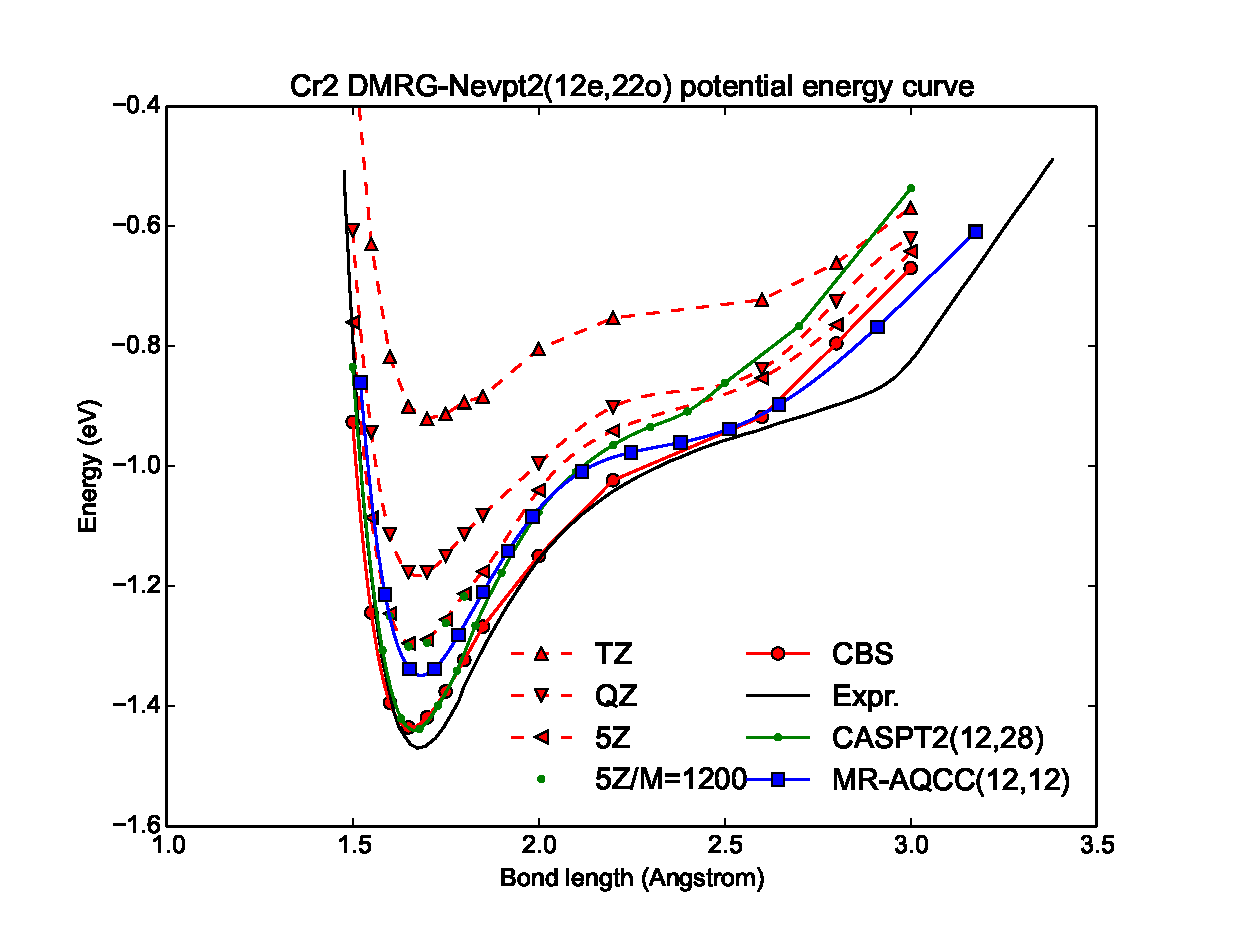
\includegraphics[width=8cm,height=6cm]{application/5qt-fitting.eps}
  \caption{DMRG-NEVPT2(12e,22o)(M=800) potential energy curve with a suite of cc-pwcVXZ (X=T,Q,5) basis set and the complete basis set (CBS) limit. The experimental curve is taken from Ref.~\onlinecite{casey_negative_1993}DMRG-CASCPT2(12e,28o) curve is from Ref.~\onlinecite{kurashige_second-order_2011} and the MR-AQCC(12e,12o) is from Ref.~\onlinecite{muller_large-scale_2009}.}
\end{figure}

Figure \ref{fig:5qt_fitting} shows the potential energy curve with a suite of cc-pwcVXZ (X=T,Q,5) basis set and the complete basis set (CBS) limit. A larger basis set gives a deeper and better curve. The CBS limit potential energy curve agreed with the experimental well, with the exception of the strong bend at about 2.8\AA, where the reliability of the RKR potential in this region has alreadybeen questioned before.\cite{roos_ground_2003}

DMRG-NEVPT2(12e,22o) results were nearly the same with DMRG-CASPT2(12e,28o)\cite{kurashige_second-order_2011} results for the $3d$ bond region. However, for the $4s$ bond (``shoulder'') region, the DMRG-NEVPT2(12e,22o) results were closer to the exerimental one, even though their CAS did not include $4p$ orbitals while DMRG-CASPT2 did. 
It is reasobalbe. Because, in the $4s$ bond region, the correlation is strong, because the $d$ orbitals are not well bonded and nearly degenerate. The Fock operator, monoelectron zero order Hamiltonian in CASPT2, is not good enough. 
The comparision between DMRG-NEVPT2(12e,22o) and DMRG-CASPT2(12e,28o) also indicates, together with the fact that only $4d$ orbitals remained in the active space after orbital optimization, $4d$ orbitals are more important than $4p$ orbitals for the static correlation and the reference function.

%The calcualted $D_e$ is 1.491eV, very close to the experimental value 1.47eV \cite{casey_negative_1993}. However, the calculated bond length is shorter than experimental value. 

\begin{table}
\caption{Spectroscopic Constants for the ground state of Cr$_2$ from different methods}
  \begin{tabular}{cccc}
  \hline
      & $D_e(eV)$ & $R_0($\AA$)$ & $\omega_e$ \\
  \hline
  DMRG-NEVPT2(12e,22o) & 1.436 & 1.656 & 476 \\ 
  DMRG-CASPT2(12e,28o)\footnote{DMRG-CASPT2(12e,28o)/{\bf $g_1$}($M=\infty$) in Ref.~\onlinecite{kurashige_second-order_2011}} & 1.61 & 1.681 & 480 \\
  MR-AQCC(12e,12o)\footnote{Ref.~\onlinecite{muller_large-scale_2009}} & 1.355 & 1.685 & 459 \\
  experiment\footnote{Ref.~\onlinecite{casey_negative_1993}} & 1.47(5) & 1.679 & 480.6(5) \\
  \hline
  \end{tabular}
\end{table}



\subsection{Poly(p-phenylene vinylene)}

Poly(p-phenylene vinylene) is a well-known light emitting conjugated polymer. It has several low-lying states that participate in its photophysics 
and has been extensively investigated with many theoretical methods, for example various semi-empirical methods~\cite{beljonne_theoretical_1995}, DMRG based on the Pariser-Parr-Pople (PPP) model Hamiltonian~\cite{lavrentiev_theoretical_1999,shukla_correlated_2002,bursill_symmetry-adapted_2009}, time-dependent density functional theory~\cite{han_time-dependent_2004} and symmetry-adapted cluster configuration interaction (SAC-CI)~\cite{saha_investigation_2007}. 
Here we examine the excited states and their energies using DMRG-SC-NEVPT2.
We limit our calculations to PPV3 (three phenyl rings) to demonstrate the capabilities of DMRG-SC-NEVPT2 for low-lying excited states in conjugated molecules.

The cc-pVDZ basis set and a (22e,22o) active space containing the 22 conjugated $\pi, \pi^*$ orbitals were used. The ground state equilibrium geometry of PPV3 was obtained via DMRG-CI geometry optimization\cite{hu_excited-state_2015}, which is implemented within an interface between \textsc{Block} and \textsc{ORCA}\cite{neese_orca_2012}, starting from the DFT/B3LYP optimized geometry. The DMRG-CI geometry optimization was first run at $M$=1000, and near convergence with $M$=2000. Canonical Hartree-Fock orbitals were used 
in the DMRG calculations in the geometry optimization.
%For the first optically bright state, we also started from the DFT guess ground state geometry.

Compared to canonical orbitals, localized orbitals usually give better convergence in DMRG calculations.~\cite{olivares-amaya_ab-initio_2015} Therefore, further state-averaged DMRG-CI calculations were carried out for the 6 lowest singlet states, using split-localized orbitals (where the occupied and unoccupied $\pi$, $\pi*$ orbitals are separately localized with the Pipek-Mezey method\cite{pipek_fast_1989}). The energies were converged to $0.2mEh$ with a bond dimension of $M$=$3200$. The excited states were identified according to their excitation signature from the ground state through the transition 1-RDM and 2-RDM
in the canonical Hartree-Fock basis. The symmetry of the states was also determined by the excitation signature: as the ground-state
 is an $A_g$ state, excitations between two orbitals of different symmetries lead to a $B_u$ excited state, and excitations between two orbitals of the same symmetry lead to an $A_g$ state.

Due to the lack of $\pi-\sigma$ interaction and dynamical correlation, the energy ordering of excitations in DMRG-CI is qualitatively different
from experiment, and the state with the HOMO$\rightarrow$LUMO excitation signature was not the lowest one in energy.
To obtain the correct state ordering, dynamic correlation was further included using DMRG-SC-NEVPT2. The DMRG-CI wavefunctions were compressed
to a smaller bond dimension of $M'$=500 and 750. The difference in excitation energy from these two different $M'$ bond dimensions
in the DMRG-SC-NEVPT2 calculation was less than $0.6 meV$ (Table~\ref{table:local}), and thus the error from incomplete $M'$ can
effectively be ignored.
The excitation energy of the first bright state as computed by DMRG-SC-NEVPT2 ($3.86 eV$) now agrees well with
\textcolor{red}{the experimental number from fluorescence in XXX solvent ($3.69 eV$)}~\cite{gierschner_fluorescence_2002} (Table~\ref{table:compare}) and the first bright ($B_u$ state) is found to lie below the $2A_g$ state, as required for efficient light emission. We also find a second $B_u$ state slightly
below the $2A_g$ state in energy. The electronic signatures of the states are shown in Table~\ref{table:local}.

\begin{table}
\caption{Vertical excitation energies of PPV-3 in vacuum from different methods.}
\label{table:compare}
\begin{tabular}{ccccc}
  \hline
  \hline
State  & DMRG-SC-NEVPT2 & DMRG/PPP & SAC-CI & expt\\
\hline
$1^1B_u$ & 3.86   &3.52\footnote{\label{fn:dmrg_1999}Ref.~\onlinecite{lavrentiev_theoretical_1999}}, 3.91\footnote{Ref.~\onlinecite{shukla_correlated_2002}}, 3.751\footnote{\label{fn:dmrg_2009}Ref.~\onlinecite{bursill_symmetry-adapted_2009}}, & 3.57\footnote{Ref.~\onlinecite{saha_investigation_2007}} & 3.69\footnote{Ref.~\onlinecite{gierschner_fluorescence_2002}} \\
%$1^1B_u$ & 3.863   &3.52\footnote{\label{fn:dmrg_1999}Ref.~\onlinecite{lavrentiev_theoretical_1999}}, 3.751\footnote{\label{fn:dmrg_2009}  Ref.~\onlinecite{bursill_symmetry-adapted_2009}}, 3.88\footnote{Ref.~\onlinecite{beljonne_theoretical_1995}},3.91\footnote{Ref.~\onlinecite{shukla_correlated_2002}}, 3.68\footnote{Ref.~\onlinecite{gierschner_fluorescence_2002}} & 3.69\footnote{Ref.~\onlinecite{gierschner_fluorescence_2002}} \\
$2^1A_g$ & 4.66   &4.06\footref{fn:dmrg_1999}, 4.618\footref{fn:dmrg_2009}& & \\
\hline
\hline
\end{tabular}
\end{table}




\begin{table*}
  \centering
  \caption{Excitation energy (eV) calculated from DMRG-SC-NEVPT2 ($M'$=500, 750) with localized orbitals.
    Excitations energies of DMRG-CI ($M$=3200) also shown for comparison. The transition signatures are calculated from the
    DMRG-CI wave function with $M$=750. The excitation coefficient of the transition $i\rightarrow j$ ($i,j \rightarrow k,l$) is given by $\bra{\Psi}a^\dagger_j a_i\ket{1^1A_g}$ ( $\bra{\Psi}a^\dagger_l a^\dagger_k a_j a_i\ket{1^1A_g}$).
The transition labels $n\rightarrow m'$ are as follows: 1, 2, 3 \ldots denote HOMO, HOMO-1, HOMO-2 \ldots canonical orbitals, while $1'$, $2'$, $3'$ \ldots denote LUMO, LUMO+1,LUMO+2 canonical orbitals. \textcolor{red}{2 d.p. sufficient!}}
  \label{table:local}
  \begin{tabular}{ccccc}
    \hline
\hline
symmetry & excitation signature &  $M'$=500 & $M'$=750 & DMRG-CI($M$=3200) \\

\hline
$1^1B_u$ & $(1\rightarrow1')$ & 3.8628   &   3.8625   & 5.1311 \\
  $2^1B_u$ & 0.71 ($5\rightarrow 1'$) + 0.66 (1$\rightarrow 3'$) & 4.4980   &   4.4978   & 4.4952    \\
  $2^1A_g$ & 0.49 ($2\rightarrow 1'$) + 0.42 (1$\rightarrow 2'$) & 4.6634   &   4.6634   & 4.8454    \\
  &   + 0.47 ($1,1\rightarrow1',1'$)  & & &\\
  $3^1B_u$ & many terms & 4.8268   &   4.8262   & 4.7541    \\
  $4^1B_u$ & many terms & 4.8441   &   4.8443   & 4.7571    \\
\hline
\hline
\end{tabular}
\end{table*}



\section{Conclusion}

In this work, we developed a general algorithm to compute different order RDMs for DMRG wave function, which can be used by many dynamic correlation methods. 
Through up to 4th order RDM, we combined DMRG and NEVPT2 to discribe static and dynamic correlations at the same time, forming DMRG-NEVPT2, 
a intruder state free second order multireference perturbation theory. 
It made the calculations complex molecules with large active spaces possible. 

To demonstrate the capability of DMRG-NEVPT2 method, we used this method to calculate the potential energy curve of chromium dimer and excited 
states of poly(p-phenylene vinylene). For chromium dimer, the extended active space included $4d$ orbitals and the so called ``double d'' effect 
were considered. It gave quantatively correct potential energy curves, demonstrating that correlation from second shell orbitals were essential for chromium dimer.
For light emitting conjugated polymers, Poly(p-phenylene vinylene), excitation energy of low-lying excited states were computed through DMRG-NEVPT2 
with different orbitals in active space. The local orbitals calculation gave results converged with bond dimension much better than canonical 
orbitals. And the accuracy from local orbital DMRG-NEVPT2 is about $0.6meV$, relative to standard NEVPT2. While the environments were not included 
in the calculations, the energy order of excited states were reasonable.

Based on above two examples, DMRG-NEVPT2 is a intruder free perturbation methods and it can be used for the molecule where large active spaces are needed.


\section*{Acknowledgements}
This work was supported by the US Department of Energy. Primary
support was provided by DE-SC0010530 and additional support
was provided by DE-SC0008624.


\bibliography{nevpt.bib}{}


\end{document}
